\section{Теоретическая часть}



\subsection{Основные вычисления}
\begin{wrapfigure}{R}{0.5\textwidth}
	\centering
	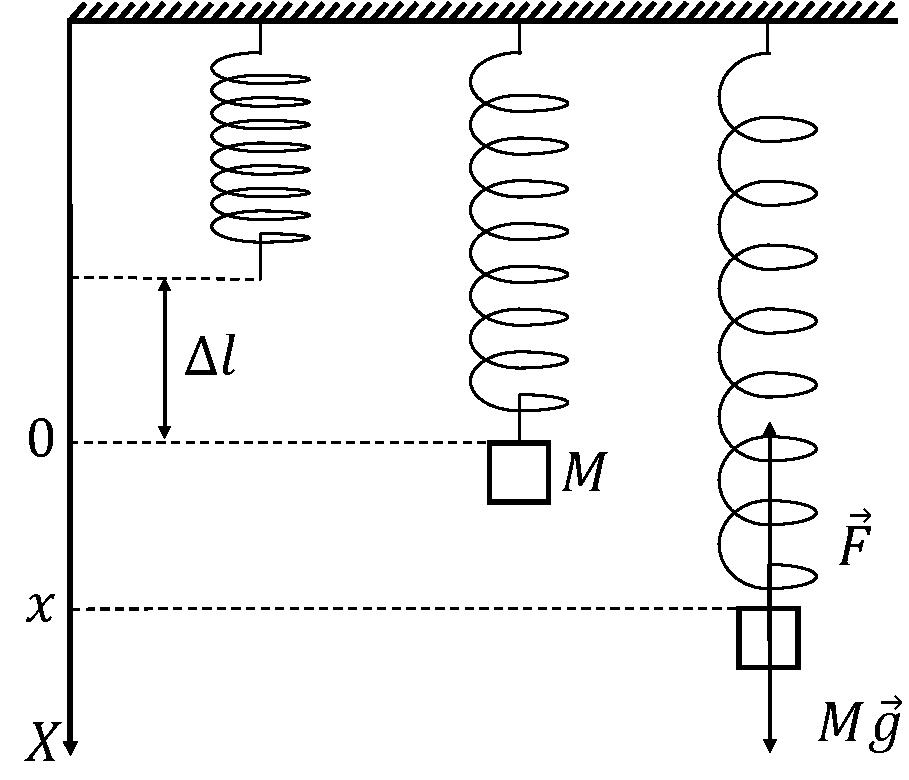
\includegraphics[width=1\linewidth]{img/ris2}
	\caption{ }
	\label{fig: 12}
\end{wrapfigure}
Равновесное положение груза массы $M$, подвешенного на пружине (см.рис.\ref{fig: 12}), определяется равенством величин силы упругости $F = k \triangle l$ и силы тяжести $Mg$.


\begin{equation}
	\label{eqution:1}
	k \triangle l = Mg
\end{equation}

, где $k$ - коэффициент упругости (жесткость) пружины, $\triangle l$ - ее удлинение от недеформированного состояния. Выведенной из положения равновесия груз колеблется около этого положения по синусоидальному (гармоническому) закону. 
\begin{equation}
	\label{eqution:2}
	x = Acos(\omega t + \varphi) 
\end{equation}

, где $x$ - смещение груза от положения равновесия, $А$ - амплитуда колебаний (величина наибольшего смещения груза от положения равновесия), $\varphi$ - начальная фала колебаний, $\omega$ - круговая (циклическая) частота, период колебаний $T = \frac{2 \pi}{\omega}$. Величины $A$ и $\varphi$ определяется на начальных условий, т.е. значениям $x$ и $V_x = \dot{x}$ в момент времени $t = 0$. Другими словами, $A$ и $\varphi$ определяются способами возбуждения колебаний груза.
Гармоническая зависимость $x(t)$ вида \ref{eqution:2} является, как можно проверить непосредственной подстановкой, решением уравнения.
\begin{equation}
	\label{eqution:3}
	\ddot{x} + \omega ^ 2 x = 0
\end{equation} 

называемого уравнением гармонического осциллятора. Кроме груза на пружине, гармоническими осцилляторами являются, например, математический маятник, электрический колебательный контур без потерь и ряд других систем.
В нашем случае уравнение \ref{eqution:3} можно получить из второго закона Ньютона, который в проекции на ось $x$ (см.рис.) имеет вид.
\begin{equation}
	\label{eqution:4}
	Ma_x = Mg + F_x
\end{equation}

Деформация пружины в произвольном положении груза равна $x + \triangle l$ ($x + \triangle l < 0$ в соответствует сжатой пружине), и проекция силы, действующей на груз со стороны пружины, равна $F_x = -k(x + \triangle l)$. Если, кроме того, учесть условие (\ref{eqution:1}) и равенство $a_x = \ddot{x}$, то после преобразований получается уравнение гармонического осциллятора.
\begin{equation}
	\label{eqution:5}
	\ddot{x} + \frac{k}{M} x = 0 
\end{equation}

Сравнение (\ref{eqution:3}) и (\ref{eqution:5}) показывает, что $\omega ^2 = \frac{k}{M}$, а период колебаний. Формула (\ref{eqution:6}) справедлива, если масса пружины $m << M$.
\begin{equation}
	\label{eqution:6}
	T = 2 \pi \sqrt{\frac{M}{k}}
\end{equation}

Выразим из формулы \ref{eqution:1} коэффициент $k$.
\begin{equation}
	\label{eqution:7}
	k = \frac{Mg}{\triangle l} = \frac{Mg}{l - l_0}
\end{equation}

\subsection{Вычисления погрешностей}

Вычислим косвенную погрешность формулы \ref{eqution:7}. Т.к. измерение длины пружинки проводились только один раз, то будем считать абсолютную погрешность равной приборной ($k_{\text{случайная}} = 0$). 

\begin{equation}
	\label{eqution: 8}
	\triangle k = \sqrt{(\frac{\mathrm d k}{\mathrm d l})^2 \triangle l^2 + (\frac{\mathrm d k}{\mathrm d l_0})^2 \triangle l_0^2 + (\frac{\mathrm d k}{\mathrm d M})^2 \triangle M^2}
\end{equation}
\begin{equation}
	\label{eqution: 9}
	\triangle k = \frac{g}{l - l_0} \sqrt{\triangle M^2 + M^2 \frac{\triangle l_0^2 + \triangle l^2
		}{(l - l_0)^2}}
\end{equation}

Измерения каждого параметра проводятся только один раз, поэтому будем считать случайную погрешность равной 0 ($\triangle l_{\text{сл}} = 0$, $\triangle l_{\text{0 сл}} = 0$, $\triangle M_{\text{сл}} = 0$).
\begin{equation}
	\label{eqution: 12}
	\triangle l = \triangle l_{\text{пр}} = t_{\alpha, \infty} * \frac{\delta _l}{3}
\end{equation}
\begin{equation}
	\label{eqution: 13}
	\triangle l_0 = \triangle l_{\text{0 пр}} = t_{\alpha, \infty} * \frac{\delta _{l}}{3}
\end{equation}
\begin{equation}
	\label{eqution: 17}
	\triangle M = \triangle M_{\text{пр}} = t_{\alpha, \infty} * \frac{\delta _{M}}{3}
\end{equation}


Для нахождения периода колебаний пружинного маятника нужно найти отношение общего времени движения от количество полных колебаний.
\begin{equation}
	\label{eqution: 10}
	T = \frac{t}{n}
\end{equation}

Вычислим абсолютную погрешность $t$.
\begin{equation}
	\label{eqution: 20}
	\triangle t_{\text{пр}} = t_{\alpha, \infty} * \frac{\delta _t}{3}
\end{equation}
\begin{equation}
	\label{equation: 11}
	S_{t, n} = \sqrt{\frac{\sum_{i = 1}^{n} (t_{\text{ср}} - t_i)^2}{n(n-1)}}
\end{equation}
\begin{equation}
	\label{eqution: 25}
	\triangle t_{\text{сл}} = t_{\alpha, n} * S_{t, n}
\end{equation}
\begin{equation}
	\label{equation: 10}
	\triangle t = \sqrt{\triangle t_\text{пр} ^2 + \triangle t_\text{сл} ^2}
\end{equation}


Вычислим косвенную погрешность формулы \ref{eqution: 10} и ее квадрата ($T^2 = T^*$).
\begin{equation}
	\label{eqution: 11}
	\triangle T = \sqrt{(\frac{\mathrm d T}{\mathrm d t})^2 \triangle t^2} = \frac{\triangle t}{n}
\end{equation}
\begin{equation}
	\label{eqution: 16}
	\triangle T^* = \sqrt{(\frac{\mathrm d T^2}{\mathrm d T})^2 * \triangle T^2} = 2T \triangle T = \frac{2T \triangle t}{n}
\end{equation}

Квадрат периода колебаний пружинного маятника также можно найти через формулу \ref{eqution:6}, возведя ее в части в квадрат.
 
\begin{equation}
	\label{eqution: 23}
	T^* = \frac{4 \pi ^2 M}{k}
\end{equation}

Выразим косвенную погрешность формулы \ref{eqution: 23}.
\begin{equation}
	\label{eqution: 24}
	\triangle T^* = \sqrt{(\frac{\mathrm d T^*}{\mathrm d k})^2 * \triangle k^2 + (\frac{\mathrm d T^*}{\mathrm d M})^2 * \triangle M^2} = \frac{4 \pi ^2 \sqrt{\triangle M^2 k^2 + \triangle k^2 M^2}}{k^2}
\end{equation}

